% Tamaño de letra.
\documentclass[12pt,titlepage]{article}
%\documentclass{article}

%------------------------------ Paquetes ----------------------------------

% Paquetes:

\usepackage[T1]{fontenc}

%Para comentarios multilínea.
\usepackage{verbatim}

% Para tener cabecera y pie de página con un estilo personalizado.
\usepackage{fancyhdr}

% Codificación UTF-8
\usepackage[utf8]{inputenc}

% Tipografía
\usepackage{palatino} % Esta es genial!
\linespread{1.05} % Palatino queda mejor con un poco más de interlineado.
%\usepackage{times} % Times New Roman.


% Castellano.
\usepackage[spanish]{babel}

% Tamaño de página y márgenes.
\usepackage[a4paper,left=2cm,right=2cm,headheight=16pt]{geometry}
%\usepackage[left=2cm,top=3cm,right=2cm,bottom=1cm,head=1.5cm,includefoot]{geometry}

% Para \href y \url
\usepackage[pdfauthor   ={Demian Ferreiro}%
           ,pdftitle    ={Trabajo Práctico - Teoría de Lenguajes}%
]{hyperref}
\hypersetup{
colorlinks=true,
linkcolor=black,
pdfborder= 0 0 0
}

% Gráficos:

% Para generar pdf.
\usepackage[pdftex]{graphicx}
\usepackage{float}
\usepackage{pdfpages}

% Para captions.
\usepackage{caption}

% Sarpadísima tipografía para listings y \texttt
\usepackage{inconsolata}

\usepackage{xcolor}

% Para ejemplos de código.
\usepackage{listings}
\lstset{language=Oz
  ,basicstyle=\ttfamily\small % Usa inconsolata
  ,identifierstyle=\ttfamily
  ,keywordstyle=\color[rgb]{0,0,1}
  ,commentstyle=\color[rgb]{0.133,0.545,0.133}
  ,stringstyle=\color[rgb]{0.627,0.126,0.941}
  ,morekeywords={true,false}
  ,showstringspaces=false     % No muestra underscores en los espacios de los strings.
  ,backgroundcolor=\color{blue!10} % Un color suave de fondo (menos chocante que el frame=single)
  ,breaklines=false            % Wrappea las lineas automáticamente.
  ,belowskip=0pt               % Reduce el espacio entre un listing y el párrafo siguiente
  ,inputencoding=utf8
  ,literate={á}{{\'a}}1
           {é}{{\'e}}1
           {í}{{\'i}}1
           {ó}{{\'o}}1
           {ú}{{\'u}}1
  %frame=single               % Un recuadro en los listings.
}

% Para fórmulas matemáticas.
\usepackage{amssymb,amsmath}

% Para pseudocódigo. Instalar texlive-science.
\usepackage{algorithmic}
\usepackage{algorithm}

% Para poder hacer \begin{Verbatim}[samepage=true]
\usepackage{fancyvrb}


% Son necesarios?
%\usepackage{float}

%------------------------------ ~paquetes ---------------------------------

%------------------------- Inicio del documento ---------------------------

\begin{document}

% ---------------------- Encabezado y pie de página -----------------------

% Encabezado: sección a la derecha.
% Pie de página: número de página a la derecha.

\pagestyle{fancy}
\renewcommand{\sectionmark}[1]{\markboth{}{\thesection\ \ #1}}
\lhead{}
\chead{}
\rhead{\rightmark}
\lfoot{}
\cfoot{}
\rfoot{\thepage}

% ---------------------- ~Encabezado y pie de página ----------------------

% -------------------------- Título y autor(es) ---------------------------

\title{Prolog}
\author{}

% -------------------------- ~Título y autor(es) --------------------------

% ------------------------------- Carátula --------------------------------

\begin{titlepage}

\thispagestyle{empty}

% Logo facultad.
\begin{center}

\includegraphics[scale=0.55]{./fiuba}\\
\textsc{\Large Universidad de Buenos Aires}\\[0.2cm]
\textsc{\Large Facultad de Ingeniería}\\[1.5cm]

% Título central.

\textsc{\large Teoría de Lenguajes (75.31)} \\[0.3cm]
\textsc{\large Trabajo Práctico} \\[0.5cm]

\rule{\linewidth}{0.5mm} \\[0.4cm]
{\huge \bfseries Trenes: Playa de maniobras} \\
%{\Large \bfseries Introducción al lenguaje y a la programación lógica}
\rule{\linewidth}{0.5mm} \\[1cm]

\vfill

\Large 
\begin{tabular}{lll}
Demian Ferrerio & 88443 & epidemian@gmail.com \\[0.5cm]
\end{tabular}

% Pie de página de la carátula.
{\Large \today}

\end{center}
\end{titlepage}

% ------------------------------- ~Carátula -------------------------------

% -------------------------------- Índice ---------------------------------

% Hago que las páginas se comiencen a contar a partir de aquí.
\setcounter{page}{1}

% Índice.
\tableofcontents
\newpage

% -------------------------------- ~Índice --------------------------------

% ----------------------------- Inicio del tp -----------------------------

\clearpage	

% Saca la indentación de los párrafos y añade un espacio entre cada uno.
\setlength{\parindent}{0pt}
\setlength{\parskip}{2ex plus 0.5ex minus 0.2ex}

% Luego del índice, links con color.
\hypersetup{
linkcolor=red
}

% Cosas Nuevas -----------------------------------------------------------------


\section{General}

Gracias al soporte de módulos que brinda Oz (a los que llama {\it functors}), el diseño de la solución pudo plantearse en distintas partes, cada una dedicada a resolver un subdominio del problema general.

\subsection{Archivos}

Los módlos de la solución se mapean en forma directa a archivos en el directorio \verb|src| del proyecto. Éstos archivos son:

\begin{itemize} 
  \item \verb|Lista.oz|: define las funciones para trabajar con listas utilizadas en el resto de la aplicación.
  \item \verb|Trenes.oz|: tiene las funciones para el manejo de trenes y sus movimientos.
  \item \verb|PruebasLista.oz|: las pruebas del módulo \verb|Lista|.
  \item \verb|PruebasTrenes.oz|: las pruebas del módulo \verb|Trenes|.
  \item \verb|Prueba.oz|: las funciones básicas para hacer pruebas.
  \item \verb|Visualizador.oz|: las funciones para visualizar gráficamente los trenes y sus movimientos.
  \item \verb|TrenesPrincipal.oz|: el punto de entrada de la aplicación.
  \item \verb|makefile.oz|: archivo utilizario usado para compilar el proyecto.
\end{itemize}

\subsection{Cómo Compilar y Ejecutar}

Para compilar el proyecto, básta con ejecutar desde la linea de comandos, sobre el directorio \verb|src|:
\begin{lstlisting}
$ ozmake
\end{lstlisting}

Esto generará los archvios \verb|.ozf|, los functors, correspondientes a cada archivo \verb|.oz|.

Una vez compilado, la aplicación puede ejecutarse con:
\begin{lstlisting}
$ ozengine TrenesPrincipal.ozf
\end{lstlisting}

Las prubeas, a su vez, pueden ejecutarse de forma análoga:
\begin{lstlisting}
$ ozengine PruebasLista.ozf
$ ozengine PruebasTrenes.ozf
\end{lstlisting}

\subsection{Herramientas Utilizadas}

Para la realización del trabajo práctico se utilizó:
\begin{itemize}
  \item {\bf Mozart/Emacs} Para codificar y hacer pruebas interactivas.
  \item Las herramientas de linea de comandos de Mozart: {\bf ozmake} y {\bf ozengine} para compilar y ejecutar las pruebas automáticas y el programa principal.
  \item El visualizador de Peter Van Roy y colaboradores\footnote{\url{http://www.info.ucl.ac.be/people/PVR/ds/CS2104/Assignments/Visualizer.zip}} para algunas pruebas interactivas y para mejor presentación del trabajo.
  \item {\bf \LaTeX} para la redacción de éste informe.
\end{itemize}

\section{Pruebas}

Una de las ventajas de programar en el paradigma funcional es la facilidad con la que se pude probar el código. Al no tener estado mutable, o {\it side effect}, hacer ``TDD'' ({\it Test Driven Development}) se reduce a especificar la salida esperada de una función dados algunos valores de sus parámetros.

\subsection{Módulo de Pruebas}

Con el fin de facilitar la definición de pruebas, se escribió un sencillo módulo utilitario de pruebas. Su definición completa es:
\lstinputlisting[basicstyle=\ttfamily\footnotesize]{../src/Prueba.oz}

Lo más importante de éste módulo es el procedimiento \lstinline|Iguales| que evalúa si dos valores, el esperado y el obtenido en una prueba, son iguales y, en caso de no serlo, imprime por pantalla un mensaje de error con la descripción de la prueba y los valores testeados.

Se puede observar que, irónicamente, en vez de utilizarse un diseño fucional puro, se optó por un diseño ``orientado a objetos'' (o, con estado). Esto se hizo así méramente para poder contar la cantidad de pruebas realizadas de una forma sencilla. Distintos paradigmas pueden resolver distintos problemas de forma más o menos ``natural''. Y así, Oz, al no forzar un paradigma determinado permite expresar una solución de la forma que más natural le resulte al programador.

\section{Listas}

\subsection{Pruebas}

Si bien la implementación de las funciones para el manejo de listas es sencilla, es conveniente escribir antes algunas pruebas que especifiquen el comportamiento esperado de las mismas.

Por ejemplo, éstas podrían ser las pruebas de la función \lstinline|Tomar|:
\begin{lstlisting}
P = {Prueba.nuevaPrueba}
L = [1 2 3 2 1]
{P.iguales {Lista.tomar L 3} [1 2 3] 'Tomar con N < Longitud'}
{P.iguales {Lista.tomar L 0} nil 'Tomar con N == 0'}
{P.iguales {Lista.tomar L 6} L 'Tomar con N > Longitud'}
\end{lstlisting}

Se puede empezar con una implementación vacía de \lstinline|tomar| \dots
\begin{lstlisting}
fun {Tomar Xs N}
   nil
end
\end{lstlisting}

\dots y ejecutar las pruebas. Estas, obviamente, fallan y nos idican qué es lo que se esperaba:
\begin{lstlisting}
$ ozengine PruebasLista.ozf
Fallo en prueba: Tomar con N < Longitud
  Se esperaba: [1 2 3]
  Pero se obtuvo: nil
Fallo en prueba: Tomar con N > Longitud
  Se esperaba: [1 2 3 2 1]
  Pero se obtuvo: nil
Pruebas exitosas/total: 2/3
\end{lstlisting}

Así, se puede ir implementando las funciones a medida que se van especificando en forma de pruebas automatizadas. 

Más importante aún, se puede escribir una implementación rápida y desprolija de una función, sólo para probar si de esa forma anda, y luego refactorizarla de una forma más prolija y elegante y coroborar que sigue andando. La confianza que se gana a la hora de refactorizar es uno de las ventajas más importantes de hacer TDD.

\subsection{Implementación}

Las funciones del módulo \lstinline|Lista| no resultan muy interesantes, ya que son bastante sencillas. Todas se basan en interar una lista recursivamente y checkear la condición de corte con pattern matching.

La implementación entera del módulo es:
\lstinputlisting[basicstyle=\ttfamily\footnotesize]{../src/Lista.oz}

\section{Trenes}

El módulo \lstinline|Trenes| tiene las funciones necesarias para el manejo de trenes y sus movimientos. Las estructuras de datos utilizadas y las funciones se implementaron de acuerdo a las pautas del enunciado.

\subsection{Aplicar Movimientos}

La función \lstinline|AplicarMovimientos| calcula los estados por los que pasa una estación de maniobras al aplicarse una lista de movimientos partiendo de un estado inicial.

\subsubsection{Pruebas}

Algunas pruebas para tener una idea de cómo debe funcionar \lstinline|AplicarMovimientos| antes de lanzarnos a codear:
\begin{lstlisting}[basicstyle=\ttfamily\footnotesize]
P = {Prueba.nuevaPrueba}
E = estado(principal:[a b] uno:nil dos:nil)
{P.iguales {Trenes.aplicarMovimientos E nil} [E] 
           'AplicarMovimientos sin movimientos'}

{P.iguales {Trenes.aplicarMovimientos E [uno(0) dos(0)]} [E E E] 
           'AplicarMovimientos con movimientos de 0 vagones'}

{P.iguales {Trenes.aplicarMovimientos E [uno(1) dos(1) uno(~1)]}
           [estado(principal:[a b] uno:nil dos:nil)
            estado(principal:[a] uno:[b] dos:nil)
            estado(principal:nil uno:[b] dos:[a])
            estado(principal:[b] uno:nil dos:[a])]
           'AplicarMovimientos con movimientos de 1 vagon'}

{P.iguales {Trenes.aplicarMovimientos E [uno(1) uno(1) uno(~1) uno(~1)]}
           [estado(principal:[a b] uno:nil dos:nil)
            estado(principal:[a] uno:[b] dos:nil)
            estado(principal:nil uno:[a b] dos:nil)
            estado(principal:[a] uno:[b] dos:nil)
            estado(principal:[a b] uno:nil dos:nil)]
           'AplicarMovimientos: los vagones deben agregarse al comienzo de'#
           ' las vías secundarias y al final de la principal'}
\end{lstlisting}

\subsubsection{Implementación}
Con el fin de mantener la complejidad del código baja, \lstinline|AplicarMovimientos| delega parte del trabajo a otras funciones:
\begin{lstlisting}[basicstyle=\ttfamily\footnotesize]
% Devuelve la lista de los estados que resulta de aplicar los movimientos Ms
% a partir del estado inicial E.
fun {AplicarMovimientos E Ms}
   case Ms of nil then [E]
   [] M|Mr then E1 = {AplicarMovimiento E M} in
      E|{AplicarMovimientos E1 Mr}
   end
end

% Devuelve el estado que resulta de aplicar el movimiento M al estado E.
fun {AplicarMovimiento E M}
   case M 
   of uno(N) then E1 = {AplicarMovimientoEnVia N E.principal E.uno} in
      estado(principal:E1.1 uno:E1.2 dos:E.dos)
   [] dos(N) then E1 = {AplicarMovimientoEnVia N E.principal E.dos} in
      estado(principal:E1.1 uno:E.uno dos:E1.2)
   end
end

% Devuelve el resultado de mover N vagones desde el tren en la vía principal 
% Ps hacia el tren en la vía secundaria Ss. El resultado es una tupla de la 
% forma <tren en la vía principal>#<tren en la vía secundaria>.
fun {AplicarMovimientoEnVia N Ps Ss}
   if N > 0 then L = {Lista.longitud Ps} - N in
      {Lista.tomar Ps L}#{Lista.agregar {Lista.eliminar Ps L} Ss}
   else
      {Lista.agregar Ps {Lista.tomar Ss ~N}}#{Lista.eliminar Ss ~N}
   end
end
\end{lstlisting}

\lstinline|AplicarMovimiento| se encarga de calcular el estado que resulta de aplicar un movimiento dado a un estado inicial haciendo pattern matching con el tipo de movimiento (\emph{uno} o \emph{dos}) y a su vez delega a \lstinline|AplicarMovimientoEnVia| el trabajo de calcular cuántos vagones quedan en la vía principal y cuántos en la vía secundaria al realizar un movimiento de $N$ vagones, pudiendo ser $N$ positivo o negativo.

\subsection{Calcular Movimientos}

La función \lstinline|CalcularMovimientos| es el corazón de la aplicación. Es la que se encarga de determinar una secuencia de movimientos capaz de alterar el orden de los vagones de un tren en la vía principal para llevarlos a un orden deseado.

\subsubsection{Primer Implementación}

Una primer implementación de \lstinline|CalcularMovimientos| resulta relativamente sencilla:
\begin{lstlisting}[basicstyle=\ttfamily\footnotesize,label=lst:calcularmovimientosv1]
% Primer versión de CalcularMovimientos. No comprime.
fun {CalcularMovimientos1 Xs Ys}
   case Xs#Ys 
   of nil#nil then nil
   [] (X|Xr)#(X|Yr) then
      % Si el primer vagón ya está en la posición esperada paso al siguiente
      {CalcularMovimientos Xr Yr}
   [] !Xs#(Y|Yr) then 
      Particion = {PartirTren Xs Y}
      HaciaUno = {Lista.longitud Particion.2} + 1
      HaciaDos = {Lista.longitud Particion.1}
      Xr = {Lista.agregar Particion.2 Particion.1}
   in
      uno(HaciaUno)
      |dos(HaciaDos)
      |uno(~HaciaUno)
      |dos(~HaciaDos)
      |{CalcularMovimientos Xr Yr}
   end
end
\end{lstlisting}

Es la típica solución recursiva con pattern matching, excepto que el matcheo se hace contra dos listas: el estado actual del tren en la vía principal, \lstinline$Xs$; y el estado al que se quiere llegar, \lstinline$Ys$. En cada llamada recursiva \lstinline|CalcularMovimientos| añade tres movimientos más a la solución, los cuales se encargan de posicionar el primer vagón de \lstinline$Ys$, \lstinline$Y$, al comienzo de la vía principal. La llamada recursiva se hace, entonces, sobre el resto de los vagones de la secuencia buscada, \lstinline$Yr$, y el resto de los vagones que quedaron en la vía principal luego del recién acomodado, \lstinline$Xr$.

Se puede observar que esta solución ya implementa la optimización de que si el primer vagón en la vía principal coincide con el primer vagón de la secuencia buscada no se realiza movimiento alguno para acomodarlo.

También puede observarse que el trabajo de dividir al tren \lstinline$Xs$ en dós en base al vagón \lstinline$Y$ se delega a la función \lstinline|PartirTren|.

\subsubsection{Partir Tren}

La función \lstinline|PartirTren| es muy sencilla de implementar gracias a las primitivas de listas implementadas anteriormente.
\begin{lstlisting}[basicstyle=\ttfamily\footnotesize]
% Devuelve la tupla que resulta de partir el tren Xs por el vagón Y. La tupla
% resultante tiene la forma: <vagones previos a Y>#<vagones posteriores Y>.
fun {PartirTren Xs Y}
   Pos = {Lista.posicion Xs Y}
in
   {Lista.tomar Xs Pos-1}#{Lista.eliminar Xs Pos}
end
\end{lstlisting}

\subsubsection{Compresión de Movimientos}

La función \lstinline|ComprimirMovimientos| toma una lsita de movimientos y la ``comprime'', descartando movimientos de 0 vagones y juntando movimientos consecutivos sobre la misma vía:
\begin{lstlisting}[basicstyle=\ttfamily\footnotesize]
fun {ComprimirMovimientos Ms}
   Ns = {EliminarMovimientosRepetidos {EliminarMovimientosNulos Ms}}
in
   if Ns == Ms then Ms else {ComprimirMovimientos Ns} end
end

fun {EliminarMovimientosNulos Ms} 
   case Ms of nil then nil
   [] uno(0)|Mr then {EliminarMovimientosNulos Mr}
   [] dos(0)|Mr then {EliminarMovimientosNulos Mr}
   [] M|Mr then M|{EliminarMovimientosNulos Mr}
   end
end

fun {EliminarMovimientosRepetidos Ms} 
   case Ms of nil then nil
   [] uno(N)|uno(M)|Mr then uno(N + M)|{EliminarMovimientosRepetidos Mr}
   [] dos(N)|dos(M)|Mr then dos(N + M)|{EliminarMovimientosRepetidos Mr}
   [] M|Mr then M|{EliminarMovimientosRepetidos Mr}
   end
end
\end{lstlisting}

Como a veces una secuencia de movimientos necesita de varias pasadas de compresión para quedar comprimida al máximo, \lstinline|ComprimirMovimientos| se llama recursivamente, aplicando una pasada por vez, hasta que la salida de una pasada da igual a su entrada.

Es interesante notar como el pattern matching simplifica gratamente la implementación tanto de \lstinline|EliminarMovimientosNulos| y \lstinline|EliminarMovimientosRepetidos|.

\subsubsection{Minimizar aún más los Movimientos}

La última mejora para minimizar los movimientos que sugiere el enunciado es hacer que, en vez de regresar siempre todos los vagones a la vía principal después de cada llamada a \lstinline|CalcularMovimientos|, mantenerlos en las vías secundarias e ir maniobrando entre las vías uno y dos para llevar los vagones a la principal. 

El código de \lstinline|CalcularMovimientos|, aplicando también la compresión de movimientos, cambia sustancialmente:
\begin{lstlisting}[basicstyle=\ttfamily\footnotesize]
% Devuelve la lista de movimientos necesarios para transformar el estado
% estado(principal:Xs uno:nil dos:nil) en 
% estado(principal:Ys uno:nil dos:nil)
fun {CalcularMovimientos Xs Ys}
   case Ys of nil then nil
   [] Y|Yr then
      Particion = {PartirTren Xs Y}
      HaciaUno = {Lista.longitud Particion.2} + 1
      HaciaDos = {Lista.longitud Particion.1}
      % Los primeros tres movimientos dejan Y en la vía principal y el resto
      % de los vagones en las vías uno y dos.
      Ms = uno(HaciaUno)
           |dos(HaciaDos)
           |uno(~1)
           |{CalcularMovimientosUnoYDos Particion.2 Particion.1 Yr}
   in
      {ComprimirMovimientos Ms}
   end
end

fun {CalcularMovimientosUnoYDos Us Ds Ys}
   case Ys of nil then nil
   [] Y|Yr then Particion L U1s D1s in
      if {Lista.miembro Us Y} then
         Particion = {PartirTren Us Y}
         L = {Lista.longitud Particion.1}
         U1s = Particion.2
         D1s = {Lista.agregar Particion.1 Ds}
         uno(~L)|dos(L)|uno(~1)|{CalcularMovimientosUnoYDos U1s D1s Yr}
      elseif {Lista.miembro Ds Y} then
         Particion = {PartirTren Ds Y}
         L = {Lista.longitud Particion.1}
         U1s = {Lista.agregar Particion.1 Us}
         D1s = Particion.2
         dos(~L)|uno(L)|dos(~1)|{CalcularMovimientosUnoYDos U1s D1s Yr}
      end
   end
end
\end{lstlisting}

\lstinline|CalcularMovimientos| calcula los primeros tres movimientos para llevar los vagones a las vías uno y dos y el primer vagon ordenado a la vía principal. Delega el resto del trabajo a \lstinline|CalcularMovimientosUnoYDos| y finalmente comprime los resultados.

\lstinline|CalcularMovimientosUnoYDos|, al igual que la primer implementación de \lstinline|CalcularMovimientos| (\ref{lst:calcularmovimientosv1}) calcula los movimientos para colocar un vagón ordenado de \lstinline|Ys| en la vía principal en cada llamada recursiva, pero en vez de mantener el resto de los vagones en la vía principal los mantiene en las vías uno y dos (listas \lstinline|Us| y \lstinline|Ds|).

A simple vista puede parecer que esta implementación podría incurrir en varios movimientos innecesarios. Por ejemplo, no implementa la optimización básica de no calcular movimientos si el vagón a procesar \lstinline|Y| ya se encuentra en la posición correcta. Pero resulta que esa optimización es innecesaria si se aplica la compresión de movimientos.

\subsection{Maniobrar}

Con la ayuda de las funciones anteriormente descriptas, la implmentación de la función principal del programa, \lstinline|Maniobrar|, resulta trivial:
\begin{lstlisting}[basicstyle=\ttfamily\footnotesize]
% Devuelve una lista de estados por los que tiene que pasar la playa de 
% maniobras para pasar del estado
% estado(principal:Xs uno:nil dos:nil) a
% estado(principal:Ys uno:nil dos:nil)
fun {Maniobrar Xs Ys}
   Ms = {CalcularMovimientos Xs Ys}
   E = estado(principal:Xs uno:nil dos:nil)
in
   {AplicarMovimientos E Ms}
end
\end{lstlisting}

\section{Visualizador}

\subsection{Modificaciones}

Se realizazon las modificaciones mínimas al código del visualizador de Peter Van Roy para adaptarlo al diseño del trabajo práctico. Estas modificaciones fueron:

\begin{itemize}
  \item Se metió el código dentro de un functor que sólo exporta el procedimiento \lstinline|Visualizar|.
  \item Se adaptaron los nombres de las estructuras al castellano. Esto es, cambiar ``main'' por ``principal'', ``one'' por ``uno'', etc.
  \item Se cambió el nombre del procedimiento principal ``Visualize'' a ``Visualizar''.
  \item Se cambió el nombre del título de la pantalla visualizada a ``Visualizador de Playa de Maniobras''.
\end{itemize}

Es resto del visualizador se dejó intacto, es decir, que la implementación sigue estando en inglés y sigue utilizando las funciones estándard de Oz para el manejo de listas (e.g. \lstinline|Length|, \lstinline|Nth|, \lstinline|List.forAllInd|) por más de que ello no sea acorde con el resto de la implementación del trabajo práctico. Se decidió dejar eso así porque la interfaz del módulo, después de los cambios hechos ya resulta acorde al resto del trabajo.

\section{Corridas de prueba}

\subsection{Desde la Linea de Comandos}

El functor ejecutable de la aplicación, \lstinline|TrenesPrincipal| está definido como:
\begin{lstlisting}[basicstyle=\ttfamily\footnotesize]
functor
import
   Trenes
   Visualizador
define
   Inicial = [a b c d e f g]
   Final = [c f a e g b d]
   {Visualizador.visualizar {Trenes.maniobrar Inicial Final}}
end
\end{lstlisting}

Y puede ejecutarse con:
\begin{lstlisting}
$ ozmake
$ ozengine TrenesPrincipal.ozf
\end{lstlisting}

\begin{figure}[H]
\begin{center}
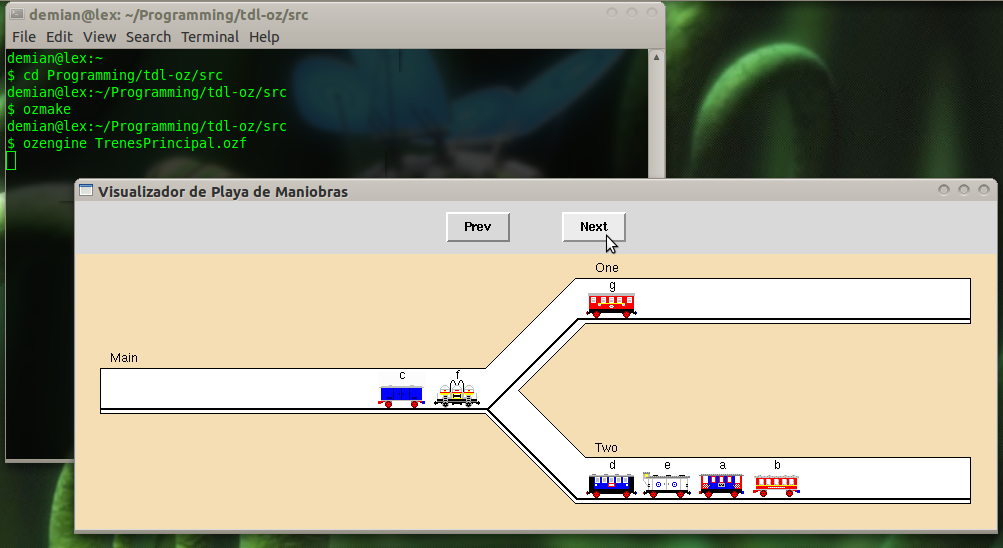
\includegraphics[width=17cm]{corrida-consola}
\caption{Corrida de prueba desde la linea de comandos.}
\end{center}
\end{figure}

\subsection{Desde Emacs}

También se puede probar la aplicación desde Emacs. Para ejecutar código en un módulo basta con cargarlo en el ambiente usando la función \lstinline|Module.link|. Una vez hecho eso, se puede programar interactivamente en Emacs y usar, por ejemplo, el browser de Oz.

\begin{figure}[H]
\begin{center}
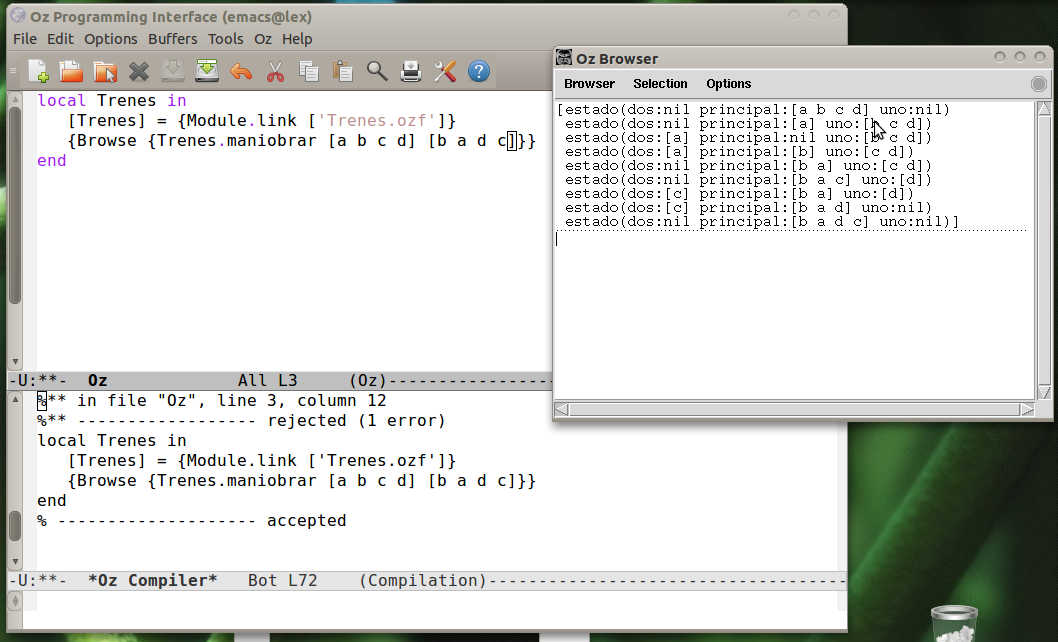
\includegraphics[width=17cm]{corrida-emacs}
\caption{Corrida de prueba desde Emacs usando el procedimiento \lstinline|Browse|.}
\end{center}
\end{figure}

% ------------------------------ Fin del tp -------------------------------

\end{document}

%---------------------------- Fin del documento ---------------------------
